\chapter{Anhang}
\label{chapter:anhang}


\begin{figure}
		\centering
		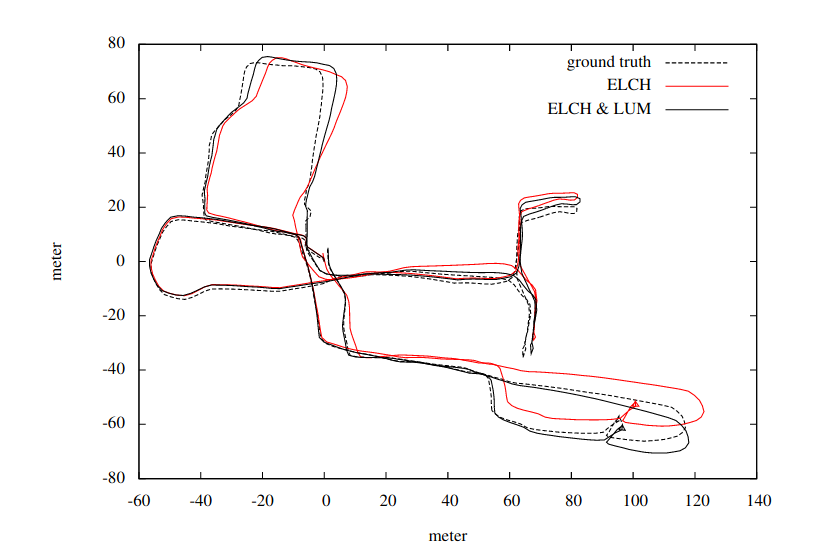
\includegraphics
			[scale=0.3]
			{elch}
		\caption
			[Caption for LOF]{Diese Grafik wurde aus \cite{sprickerhof2011heuristic} entnommen und dient als Vergleich zu den in Kapitel \ref{chapter:loop_closure} herausgearbeiteten Ergebnissen. Ein direkter, wertebasierter Vergleich mit den Ergebnissen aus \cite{sprickerhof2011heuristic} ist nicht möglich, da diese dort nur für einen anderen Datensatz angegeben sind. Ein visueller Vergleich der Ansätze zeigt aber eine deutliche Verbesserung des in dieser Arbeit vorgestellten Ansatzes im Gegensatz zum vorgeschlagenen Ansatz aus \cite{sprickerhof2011heuristic}. Nur an wenigen Stellen ist eine leicht größere Abweichung zur Ground-Truth zu erkennen. An allen anderen Stellen ist eine deutliche Verbesserung erkennbar.}                                                                                                                                     
		\label{fig:ELCH}
\end{figure}

